\section{Assembly Calculus}

\subsection{Framework}

In AC, the `brain' is modelled as a collection of \textit{areas}, each containing $n$ excitatory neurons of which at most $k \ll n$ may fire simultaneously. Areas are connected by sparse random bipartite graphs; we use a fixed in-degree $k_\mathrm{in}$ as a deterministic equivalent of the Erd\H{o}s–R\'{e}nyi model in the sparse limit. At each discrete time step, neuron $v$ computes its total synaptic input $s_v = \sum_{u \in \mathrm{src}(v)} w_{uv}\, x_u$, and $k$ neurons with the largest $s_v$ are selected (the \textit{$k$-cap} operation). The resulting binary activation pattern is the \textit{assembly}: a sparse, distributed code based on the current input (Figure~\ref{fig:ac_fundamentals}).

\begin{figure}[t]
\centering
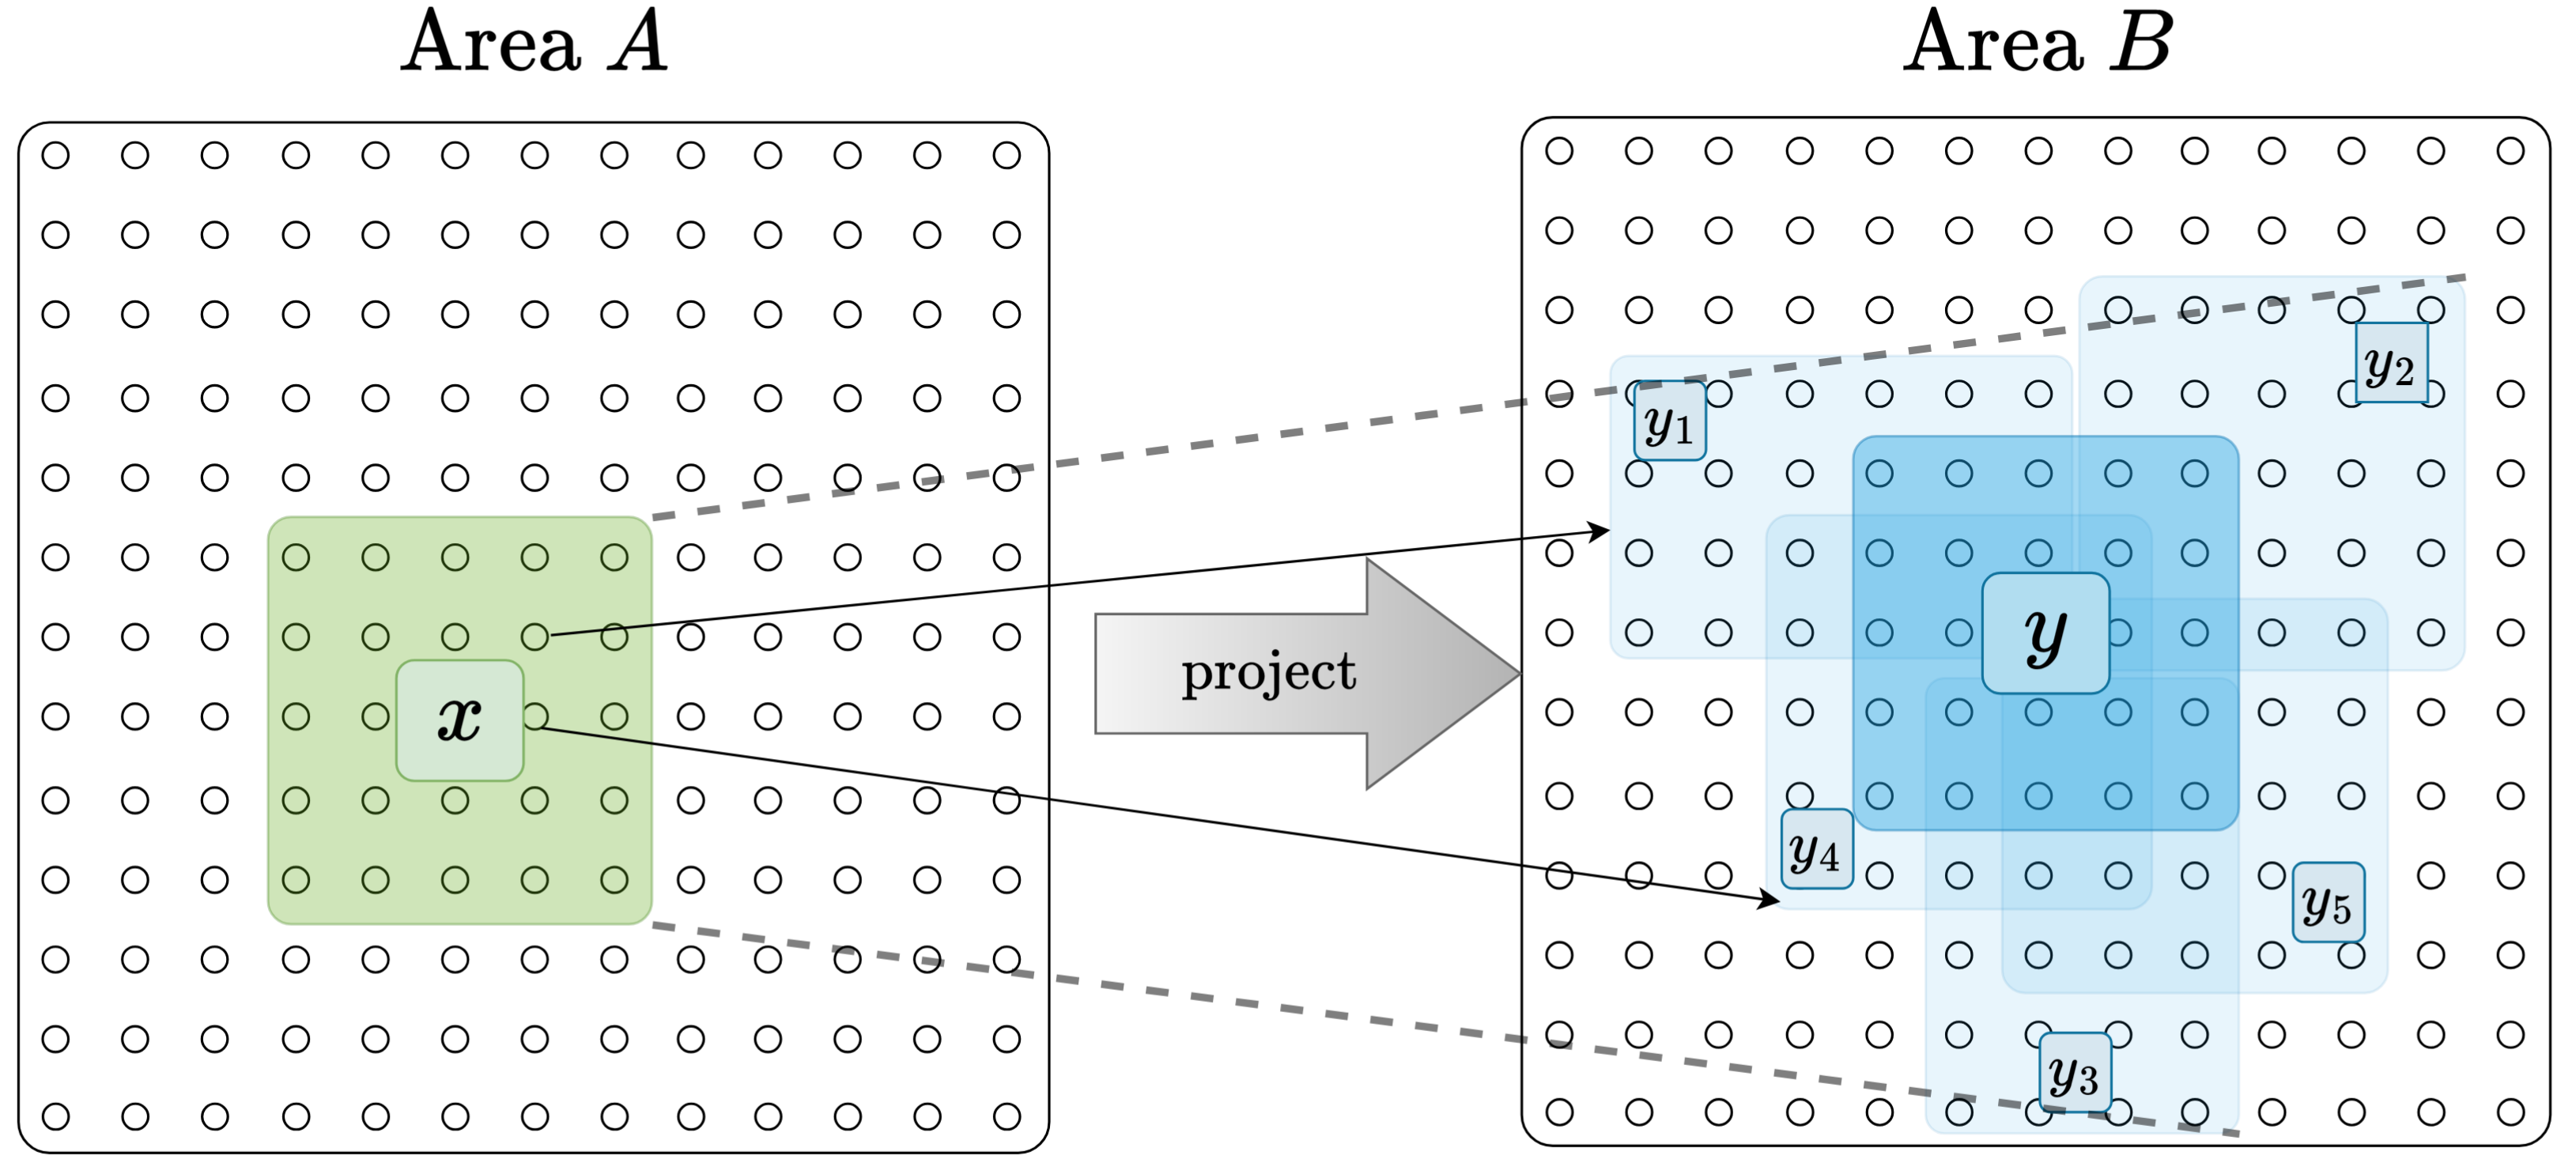
\includegraphics[width=0.9\linewidth]{figures/AC_fundamentals.png}
\caption{Fundamental \textbf{Project} operation of Assembly Calculus. Binary input vectors are projected into a neural area where the $k$-cap operation selects the top-$k$ most activated neurons to form a sparse assembly. Recurrent plasticity strengthens connections between co-active neurons, causing assemblies to stabilise over repeated presentations of the same input.}
\vspace{-10pt}
\label{fig:ac_fundamentals}
\end{figure}


The key operations are: \textit{projection}, in which stimulating an area through feedforward connections forms a new assembly in a target area; \textit{association}, in which repeated co-activation strengthens shared connections; and \textit{reciprocal stabilisation}, in which bidirectional connections between areas cause assemblies to reinforce each other. Under Erd\H{o}s--R\'{e}nyi random graph assumptions, Papadimitriou et al.\cite{papadimitriouBrainComputationAssemblies2020} showed these operations can: simulate $\mathcal{O}(nk)$ space-bounded computations. Mitropolsky et al.\cite{mitropolskyBiologicallyPlausibleParser2021}
demonstrated that hierarchical syntactic structure can emerge from assembly dynamics alone, implementing a parser for natural language using only AC operations (with pre-defined symbolic assemblies). The parser works by assigning each word a set of gate commands that control which brain areas (SUBJ, VERB, OBJ, etc.) are open for communication. As each word is read in, it projects its assembly into the appropriate open area, and the gating ensures that only grammatically valid connections form, e.g. "man" projects into SUBJ, "saw" projects into VERB while also absorbing the existing SUBJ assembly. The final parse tree is recovered by tracing which assemblies became linked through these projections.

\begin{figure*}[t]
\centering

\tikzset{
  neuron/.style={circle, draw=black!40, minimum size=7pt, inner sep=0pt, line width=0.35pt},
  active/.style={neuron, fill=black!85, draw=black!70},
  inactive/.style={neuron, fill=white},
  areabox/.style={draw=black!60, rounded corners=5pt, thick},
  arr/.style={-{Stealth[length=4pt]}, thick},
  lbl/.style={font=\scriptsize},
  sublbl/.style={font=\tiny\itshape, text=black!50},
}

\begin{tikzpicture}


\draw[-{Stealth[length=5pt]}, thick, black!40] (-1.0, 3.90) -- (13.8, 3.90)
  node[lbl, midway, above, text=black!50] {time};


\node[font=\small\bfseries] at (0, 3.55) {$t_{i{-}1}$};

\draw[rounded corners=5pt, draw=black!25, fill=gray!6]
  (-1.31, -0.79) rectangle (2.19, 2.71);
\node[font=\scriptsize, text=black!25] at (2.08, -0.68) {$\ddots$};
\draw[rounded corners=5pt, draw=black!35, fill=gray!3]
  (-1.53, -0.57) rectangle (1.97, 2.93);
\draw[areabox, fill=white] (-1.75, -0.35) rectangle (1.75, 3.15);

\fill[blue!10, rounded corners=5pt] (-1.70, 1.70) rectangle (0.20, 2.60);
\draw[blue!50, rounded corners=5pt, line width=1.2pt] (-1.70, 1.70) rectangle (0.20, 2.60);

\node[inactive] at (-1.50, 2.90) {};
\node[inactive] at (-1.00, 2.90) {};
\node[inactive] at (-0.50, 2.90) {};
\node[inactive] at ( 0.00, 2.90) {};
\node[inactive] at ( 0.50, 2.90) {};
\node[inactive] at ( 1.00, 2.90) {};
\node[inactive] at ( 1.50, 2.90) {};
\node[active]   at (-1.50, 2.40) {};
\node[active]   at (-1.00, 2.40) {};
\node[active]   at (-0.50, 2.40) {};
\node[active]   at ( 0.00, 2.40) {};
\node[inactive] at ( 0.50, 2.40) {};
\node[inactive] at ( 1.00, 2.40) {};
\node[inactive] at ( 1.50, 2.40) {};
\node[active]   at (-1.50, 1.90) {};
\node[active]   at (-1.00, 1.90) {};
\node[active]   at (-0.50, 1.90) {};
\node[active]   at ( 0.00, 1.90) {};
\node[inactive] at ( 0.50, 1.90) {};
\node[inactive] at ( 1.00, 1.90) {};
\node[inactive] at ( 1.50, 1.90) {};
\node[inactive] at (-1.50, 1.40) {};
\node[inactive] at (-1.00, 1.40) {};
\node[inactive] at (-0.50, 1.40) {};
\node[inactive] at ( 0.00, 1.40) {};
\node[inactive] at ( 0.50, 1.40) {};
\node[inactive] at ( 1.00, 1.40) {};
\node[inactive] at ( 1.50, 1.40) {};
\node[inactive] at (-1.50, 0.90) {};
\node[inactive] at (-1.00, 0.90) {};
\node[inactive] at (-0.50, 0.90) {};
\node[inactive] at ( 0.00, 0.90) {};
\node[inactive] at ( 0.50, 0.90) {};
\node[inactive] at ( 1.00, 0.90) {};
\node[inactive] at ( 1.50, 0.90) {};
\node[inactive] at (-1.50, 0.40) {};
\node[inactive] at (-1.00, 0.40) {};
\node[inactive] at (-0.50, 0.40) {};
\node[inactive] at ( 0.00, 0.40) {};
\node[inactive] at ( 0.50, 0.40) {};
\node[inactive] at ( 1.00, 0.40) {};
\node[inactive] at ( 1.50, 0.40) {};
\node[inactive] at (-1.50, -0.10) {};
\node[inactive] at (-1.00, -0.10) {};
\node[inactive] at (-0.50, -0.10) {};
\node[inactive] at ( 0.00, -0.10) {};
\node[inactive] at ( 0.50, -0.10) {};
\node[inactive] at ( 1.00, -0.10) {};
\node[inactive] at ( 1.50, -0.10) {};

\node[lbl, blue!60!black] at (0, -1.00) {$\mathbf{a}^{(t_{i-1})}$: $k$ of $n$ neurons active};

\draw[arr, black!50] (0, -1.85) -- (0, -1.15)
  node[lbl, right, pos=0.5, xshift=2pt] {$\mathbf{W}^{\mathrm{ff}}$};

\node[sublbl] at (0, -2.00) {$\mathbf{x}^{(t_{i-1})} \in \{0,1\}^{n_\mathrm{input}}$};

\node[draw=black!40, rounded corners=2pt, fill=orange!6,
      minimum width=3.5cm, minimum height=0.45cm] at (0, -2.45) {};
\fill[black!75] (-1.35, -2.60) rectangle ++(0.12, 0.30);
\draw[black!20] (-1.18, -2.60) rectangle ++(0.12, 0.30);
\fill[black!75] (-1.01, -2.60) rectangle ++(0.12, 0.30);
\fill[black!75] (-0.84, -2.60) rectangle ++(0.12, 0.30);
\draw[black!20] (-0.67, -2.60) rectangle ++(0.12, 0.30);
\fill[black!75] (-0.50, -2.60) rectangle ++(0.12, 0.30);
\node[font=\scriptsize, text=black!40] at (0.0, -2.45) {$\cdots$};
\draw[black!20] (0.50, -2.60) rectangle ++(0.12, 0.30);
\fill[black!75] (0.67, -2.60) rectangle ++(0.12, 0.30);
\fill[black!75] (0.84, -2.60) rectangle ++(0.12, 0.30);
\draw[black!20] (1.01, -2.60) rectangle ++(0.12, 0.30);
\fill[black!75] (1.18, -2.60) rectangle ++(0.12, 0.30);


\draw[arr, red!55, line width=1.6pt]
  (1.90, 1.90) -- (3.80, 1.90)
  node[lbl, above, midway, text=red!55] {$\mathbf{W}^{\mathrm{rec}} \mathbf{a}^{(t_{i-1})}$}
  node[sublbl, below, midway] {recurrent drive};


\node[font=\small\bfseries] at (5.7, 3.55) {$t_i$};

\draw[rounded corners=5pt, draw=black!25, fill=gray!6]
  (4.39, -0.79) rectangle (7.89, 2.71);
\node[font=\scriptsize, text=black!25] at (7.78, -0.68) {$\ddots$};
\draw[rounded corners=5pt, draw=black!35, fill=gray!3]
  (4.17, -0.57) rectangle (7.67, 2.93);
\draw[areabox, fill=white] (3.95, -0.35) rectangle (7.45, 3.15);

\fill[blue!5, rounded corners=5pt] (4.00, 1.70) rectangle (5.90, 2.60);
\draw[blue!35, rounded corners=5pt, line width=0.9pt, dashed] (4.00, 1.70) rectangle (5.90, 2.60);

\fill[teal!10, rounded corners=5pt] (5.00, 1.20) rectangle (6.90, 2.10);
\draw[teal!60, rounded corners=5pt, line width=1.2pt] (5.00, 1.20) rectangle (6.90, 2.10);

\node[inactive] at (4.20, 2.90) {};
\node[inactive] at (4.70, 2.90) {};
\node[inactive] at (5.20, 2.90) {};
\node[inactive] at (5.70, 2.90) {};
\node[inactive] at (6.20, 2.90) {};
\node[inactive] at (6.70, 2.90) {};
\node[inactive] at (7.20, 2.90) {};
\node[inactive] at (4.20, 2.40) {};
\node[inactive] at (4.70, 2.40) {};
\node[inactive] at (5.20, 2.40) {};
\node[inactive] at (5.70, 2.40) {};
\node[inactive] at (6.20, 2.40) {};
\node[inactive] at (6.70, 2.40) {};
\node[inactive] at (7.20, 2.40) {};
\node[inactive] at (4.20, 1.90) {};
\node[inactive] at (4.70, 1.90) {};
\node[active]   at (5.20, 1.90) {};
\node[active]   at (5.70, 1.90) {};
\node[active]   at (6.20, 1.90) {};
\node[active]   at (6.70, 1.90) {};
\node[inactive] at (7.20, 1.90) {};
\node[inactive] at (4.20, 1.40) {};
\node[inactive] at (4.70, 1.40) {};
\node[active]   at (5.20, 1.40) {};
\node[active]   at (5.70, 1.40) {};
\node[active]   at (6.20, 1.40) {};
\node[active]   at (6.70, 1.40) {};
\node[inactive] at (7.20, 1.40) {};
\node[inactive] at (4.20, 0.90) {};
\node[inactive] at (4.70, 0.90) {};
\node[inactive] at (5.20, 0.90) {};
\node[inactive] at (5.70, 0.90) {};
\node[inactive] at (6.20, 0.90) {};
\node[inactive] at (6.70, 0.90) {};
\node[inactive] at (7.20, 0.90) {};
\node[inactive] at (4.20, 0.40) {};
\node[inactive] at (4.70, 0.40) {};
\node[inactive] at (5.20, 0.40) {};
\node[inactive] at (5.70, 0.40) {};
\node[inactive] at (6.20, 0.40) {};
\node[inactive] at (6.70, 0.40) {};
\node[inactive] at (7.20, 0.40) {};
\node[inactive] at (4.20, -0.10) {};
\node[inactive] at (4.70, -0.10) {};
\node[inactive] at (5.20, -0.10) {};
\node[inactive] at (5.70, -0.10) {};
\node[inactive] at (6.20, -0.10) {};
\node[inactive] at (6.70, -0.10) {};
\node[inactive] at (7.20, -0.10) {};

\node[lbl, teal!60!black] at (5.7, -1.00) {$\mathbf{a}^{(t_i)}$};

\draw[arr, black!50] (5.7, -1.85) -- (5.7, -1.15)
  node[lbl, right, pos=0.5, xshift=2pt] {$\mathbf{W}^{\mathrm{ff}}$};

\node[sublbl] at (5.7, -2.00) {$\mathbf{x}^{(t_i)} \in \{0,1\}^{n_\mathrm{input}}$};

\node[draw=black!40, rounded corners=2pt, fill=orange!6,
      minimum width=3.5cm, minimum height=0.45cm] at (5.7, -2.45) {};
\fill[black!75] (4.35, -2.60) rectangle ++(0.12, 0.30);
\draw[black!20] (4.52, -2.60) rectangle ++(0.12, 0.30);
\draw[black!20] (4.69, -2.60) rectangle ++(0.12, 0.30);
\fill[black!75] (4.86, -2.60) rectangle ++(0.12, 0.30);
\fill[black!75] (5.03, -2.60) rectangle ++(0.12, 0.30);
\draw[black!20] (5.20, -2.60) rectangle ++(0.12, 0.30);
\node[font=\scriptsize, text=black!40] at (5.7, -2.45) {$\cdots$};
\fill[black!75] (6.20, -2.60) rectangle ++(0.12, 0.30);
\fill[black!75] (6.37, -2.60) rectangle ++(0.12, 0.30);
\draw[black!20] (6.54, -2.60) rectangle ++(0.12, 0.30);
\fill[black!75] (6.71, -2.60) rectangle ++(0.12, 0.30);
\draw[black!20] (6.88, -2.60) rectangle ++(0.12, 0.30);


\node[font=\normalsize, text=black!30] at (8.70, 1.40) {$\boldsymbol{\cdots}$};


\node[font=\small\bfseries] at (11.4, 3.55) {$t_n$};

\draw[rounded corners=5pt, draw=black!25, fill=gray!6]
  (10.09, -0.79) rectangle (13.59, 2.71);
\node[font=\scriptsize, text=black!25] at (13.48, -0.68) {$\ddots$};
\draw[rounded corners=5pt, draw=black!35, fill=gray!3]
  (9.87, -0.57) rectangle (13.37, 2.93);
\draw[areabox, fill=white] (9.65, -0.35) rectangle (13.15, 3.15);

\fill[blue!5, rounded corners=5pt] (9.70, 0.70) rectangle (11.60, 1.60);
\draw[blue!35, rounded corners=5pt, line width=0.9pt, dashed] (9.70, 0.70) rectangle (11.60, 1.60);

\fill[violet!10, rounded corners=5pt] (10.20, 0.20) rectangle (12.10, 1.10);
\draw[violet!60, rounded corners=5pt, line width=1.2pt] (10.20, 0.20) rectangle (12.10, 1.10);

\node[inactive] at (9.90, 2.90) {};
\node[inactive] at (10.40, 2.90) {};
\node[inactive] at (10.90, 2.90) {};
\node[inactive] at (11.40, 2.90) {};
\node[inactive] at (11.90, 2.90) {};
\node[inactive] at (12.40, 2.90) {};
\node[inactive] at (12.90, 2.90) {};
\node[inactive] at (9.90, 2.40) {};
\node[inactive] at (10.40, 2.40) {};
\node[inactive] at (10.90, 2.40) {};
\node[inactive] at (11.40, 2.40) {};
\node[inactive] at (11.90, 2.40) {};
\node[inactive] at (12.40, 2.40) {};
\node[inactive] at (12.90, 2.40) {};
\node[inactive] at (9.90, 1.90) {};
\node[inactive] at (10.40, 1.90) {};
\node[inactive] at (10.90, 1.90) {};
\node[inactive] at (11.40, 1.90) {};
\node[inactive] at (11.90, 1.90) {};
\node[inactive] at (12.40, 1.90) {};
\node[inactive] at (12.90, 1.90) {};
\node[inactive] at (9.90, 1.40) {};
\node[inactive] at (10.40, 1.40) {};
\node[inactive] at (10.90, 1.40) {};
\node[inactive] at (11.40, 1.40) {};
\node[inactive] at (11.90, 1.40) {};
\node[inactive] at (12.40, 1.40) {};
\node[inactive] at (12.90, 1.40) {};
\node[inactive] at (9.90, 0.90) {};
\node[active]   at (10.40, 0.90) {};
\node[active]   at (10.90, 0.90) {};
\node[active]   at (11.40, 0.90) {};
\node[active]   at (11.90, 0.90) {};
\node[inactive] at (12.40, 0.90) {};
\node[inactive] at (12.90, 0.90) {};
\node[inactive] at (9.90, 0.40) {};
\node[active]   at (10.40, 0.40) {};
\node[active]   at (10.90, 0.40) {};
\node[active]   at (11.40, 0.40) {};
\node[active]   at (11.90, 0.40) {};
\node[inactive] at (12.40, 0.40) {};
\node[inactive] at (12.90, 0.40) {};
\node[inactive] at (9.90, -0.10) {};
\node[inactive] at (10.40, -0.10) {};
\node[inactive] at (10.90, -0.10) {};
\node[inactive] at (11.40, -0.10) {};
\node[inactive] at (11.90, -0.10) {};
\node[inactive] at (12.40, -0.10) {};
\node[inactive] at (12.90, -0.10) {};

\node[lbl, violet!60!black] at (11.4, -1.00) {$\mathbf{a}^{(t_n)}$};

\draw[arr, black!50] (11.4, -1.85) -- (11.4, -1.15)
  node[lbl, right, pos=0.5, xshift=2pt] {$\mathbf{W}^{\mathrm{ff}}$};

\node[sublbl] at (11.4, -2.00) {$\mathbf{x}^{(t_n)} \in \{0,1\}^{n_\mathrm{input}}$};

\node[draw=black!40, rounded corners=2pt, fill=orange!6,
      minimum width=3.5cm, minimum height=0.45cm] at (11.4, -2.45) {};
\draw[black!20] (10.05, -2.60) rectangle ++(0.12, 0.30);
\fill[black!75] (10.22, -2.60) rectangle ++(0.12, 0.30);
\fill[black!75] (10.39, -2.60) rectangle ++(0.12, 0.30);
\draw[black!20] (10.56, -2.60) rectangle ++(0.12, 0.30);
\fill[black!75] (10.73, -2.60) rectangle ++(0.12, 0.30);
\fill[black!75] (10.90, -2.60) rectangle ++(0.12, 0.30);
\node[font=\scriptsize, text=black!40] at (11.4, -2.45) {$\cdots$};
\fill[black!75] (11.90, -2.60) rectangle ++(0.12, 0.30);
\draw[black!20] (12.07, -2.60) rectangle ++(0.12, 0.30);
\fill[black!75] (12.24, -2.60) rectangle ++(0.12, 0.30);
\fill[black!75] (12.41, -2.60) rectangle ++(0.12, 0.30);
\draw[black!20] (12.58, -2.60) rectangle ++(0.12, 0.30);

\end{tikzpicture}

\caption{Inside a per-class RecurrentArea $c$ over a period of $n$ frames. $C$ independent areas (one per class) process the same input in parallel. Each neuron receives feedforward drive from the current input $\mathbf{x}^{(t)}$ plus recurrent drive from the previous assembly $\mathbf{a}_{c}^{(t{-}1)}$; the top-$k$ neurons fire ($k$-cap). Plasticity strengthens co-active feedforward and recurrent edges, causing each area to learn class-specific spectro-temporal trajectories. The area with learned dynamics that best match the input (highest resonance score $R_c$) determines the predicted class.}
\vspace{-10pt}
\label{fig:assembly_detail}
\end{figure*}


\subsection{Temporal Dynamics}

Extending AC to sequential processing, Dabagia et al.\cite{dabagiaComputationSequencesAssemblies2024}
 showed that recurrent connections within an area naturally give rise to \textit{synfire chains}: when a sequence of stimuli is presented repeatedly, assemblies form at each position and forward recurrent weights strengthen, resulting in \textit{pattern completion}, i.e., sequence recall from partial input.

A serious challenge for sequential computation is \textit{transition disambiguation}: when the same stimulus recurs at different positions in a sequence, the system must produce different successors depending on context. \textit{Refractory adaptation} \cite{dabagiaComputationSequencesAssemblies2024}
solves this: neurons that fire accumulate an input-proportional negative bias that suppresses their future activation. Sequence learning with refractory adaptation create a discrete-time dynamical system, with the trajectory through assembly space depending on the full history of prior activations, not just the current input.


\subsection{Plasticity Rules}

Weights are updated after each $k$-cap step by a local plasticity rule. In this paper we use standard Hebbian learning~\cite{hebbOrganizationBehaviorNeuropsychological1949}: for each edge $e$ with weight $w_e$ where both pre- and post-synaptic neurons are active,
\begin{equation}\label{eq:hebbian}
    w_e \leftarrow w_e(1{+}\beta)
\end{equation}
where $\beta$ is the learning rate, followed by per-destination normalisation. All weight updates are purely local, depending only on pre- and post-synaptic activity per-edge.

Standard Hebbian learning only strengthens co-active connections, relying entirely on renormalisation to implicitly weaken others. This can cause assemblies to merge over time, as inactive-presynaptic connections to winning neurons are never explicitly penalised. To address this, we additionally employ a variant of the ABS (Artola--Br\"ocher--Singer) plasticity rule ~\cite{Artola1990-gk}~\cite{garagnaniRecruitmentConsolidationCell2009}, which adds \textit{heterosynaptic long-term depression} (LTD): when a postsynaptic neuron fires but a presynaptic neuron did not contribute, that connection is weakened:
\begin{equation}\label{eq:abs}
    w_e \leftarrow \begin{cases}
        w_e(1{+}\beta) & \text{if pre and post active (LTP)} \\
        w_e(1{-}\beta) & \text{if pre inactive, post active (LTD)} \\
        w_e & \text{otherwise}
    \end{cases}
\end{equation}
followed by clamping $w_e \geq 0$ and per-destination normalisation. This competitive mechanism ensures that winning neurons strengthen only the connections that actually drove them, while explicitly weakening irrelevant inputs.


Within AC models, information is encoded in sparse neuronal assemblies that can be created, re-used, and combined into sequences~\cite{dabagiaComputationSequencesAssemblies2024}. This provides a natural route to compositionality: assemblies can stand in for phone- or word-like units, and their flexible recombination can in principle support an open vocabulary. Finally, the core operations of AC, such as projection between areas, association through co-activation, and stabilisation via recurrent feedback, give rise to rich temporal dynamics and sequence completion~\cite{dabagiaComputationSequencesAssemblies2024}. These properties make AC-based models an interesting framework for constructing speech processing systems.
